\chapter{Rectifier}
\section{Theory and related work} \label{sec:literature_rectifier}
The half wave rectifier was chosen for this design and can be seen in Figure \ref{fig:rectifierdiagram}, this was chosen as it is requires less diodes than a full wave rectifier, however since it only conducts every positive half cycle a bigger smoothing capacitor is required.


\section{Design} \label{sec:design_rectifier}
Firstly a suitable output voltage, allowable output voltage ripple as well as a maximum load requirement had to be chosen. The maximum input voltage was chosen as $\SI{24}{V_{RMS}}$ and a ripple of $50\%$ was chosen, it is worth noting that from \cite{1n4007:2011} the voltage drop over the diode was found as $\SI{1}{V}$ which meant that the output voltage of the rectifier would always be $\SI{1}{V}$ less than the peak value of the sinusoidal input. As the \SI{5}{V} power supply was designed to require no more than \SI{100}{\milli A} and the \SI{-5}{V} power supply no more than \SI{150}{\milli A} a full load of $\SI{250}{\Omega}$ was used. Referring to the 1N4007 diode datasheet it was confirmed that the full load current draw did not exceed the $\SI{1}{A}$ maximum forward current of the diode. Using Equation \ref{eq:rectifierripple} from \cite{Neaman:2018} the required capacitor was found to be \SI{222.22}{\micro F}, thus a \SI{220}{\micro F} was chosen.

\begin{equation}
   V_{r} = \frac{V_{m}}{fRC}
   \label{eq:rectifierripple}. 
\end{equation}

\begin{figure}
    \centering
    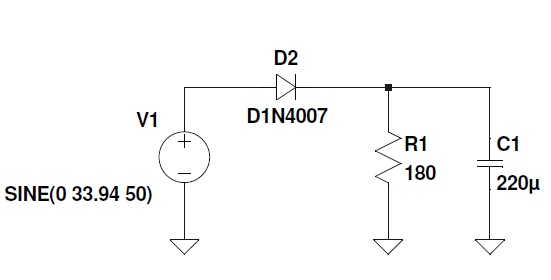
\includegraphics[width = 0.4\linewidth]{Figures/rectifier.jpg}
    \caption{Rectifier design with $\SI{24}{V_{RMS}}$ input}
    \label{fig:rectifierdiagram}
\end{figure}

\section{Simulation} \label{sec:simulation_rectifier}
The rectifier circuit was simulated with both $\SI{24}{V_{RMS}}$ and $\SI{18}{V_{RMS}}$ inputs. With the voltage ripple given a $\SI{18}{V_{RMS}}$ input shown in Figure \ref{subfig:18Vsim}. For a $\SI{24}{V_{RMS}}$ input a ripple of $34.5\%$ was reported, and for a $\SI{18}{V_{RMS}}$ input a ripple of $34.8\%$ was reported, which was below the maximum ripple designed for. 

\begin{figure}
 \centering
     \begin{subfigure}[]{0.45\textwidth}
        \centering
         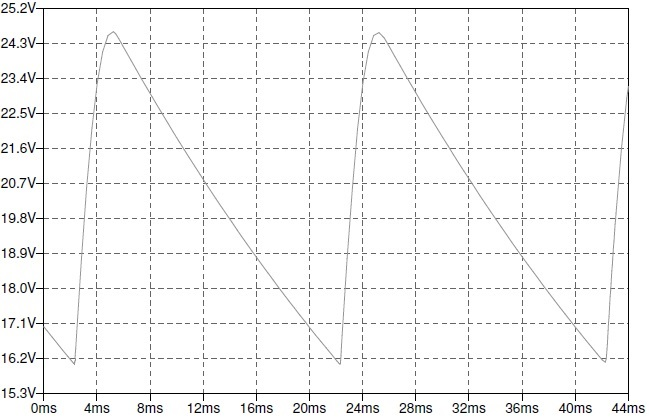
\includegraphics[width=1\linewidth]{./Figures/rectifier18vplot.jpg}
		    \caption{SPICE simulated output} \label{subfig:18Vsim}
     \end{subfigure}
      \begin{subfigure}[]{0.45\textwidth}
              \centering
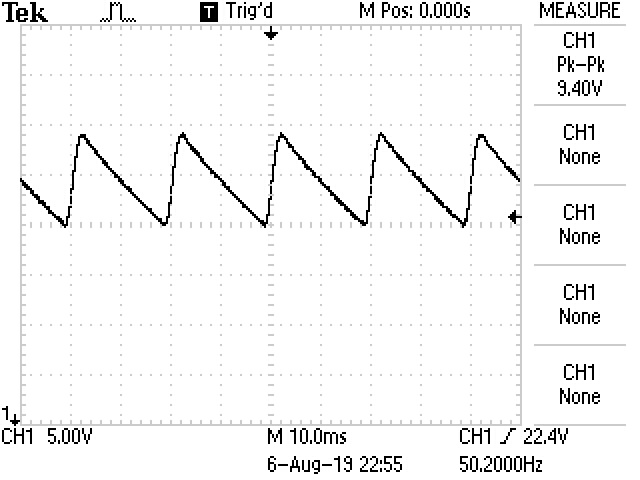
\includegraphics[width=1\linewidth]{./Figures/rectifier18vmeas.JPG}
		    \caption{Output measured in laboratory}  \label{subfig:18Vmeas}
     \end{subfigure}
   \caption[Rectifier Output Voltage Ripple]{Rectifier Output Voltage Ripple. (a) Simulated output, (b) Measured output}
    \label{fig:regulator_simulation_results_box}
 \end{figure}

\section{Measurements} \label{sec:measurements_rectifier}
The circuit was then built and the output was measured with a full load of $\SI{250}{\Omega}$. This output voltage was then measured against an input voltage of both $\SI{18}{V_{RMS}}$ and $\SI{24}{V_{RMS}}$. The ripple given a $\SI{18}{V_{RMS}}$ input can be seen in Figure \ref{subfig:18Vmeas}. Given both inputs a maximum ripple of only $36.9\%$ was reported, which was far below the maximum ripple designed for. This allowed for a continuous current supply to all of the subcircuits and did not exceed the minimum voltage requirements of the switch mode power supply. These measurements agreed with the results that were obtained in SPICE and confirmed the design of the regulator.

